\documentclass[tikz,crop,border=0.25cm]{standalone}

\usepackage{tikz}
\usetikzlibrary{calc,shapes,arrows,fit}

\tikzset{
	node distance=3.5cm,
	auto,
	>=latex',
	punkt/.style={
		rectangle,
		draw=black,
		semithick,
		text width=6.5em,
		minimum height=2.75em,
		text centered
	}
}

\begin{document}
	\pagestyle{empty}
	\sffamily
	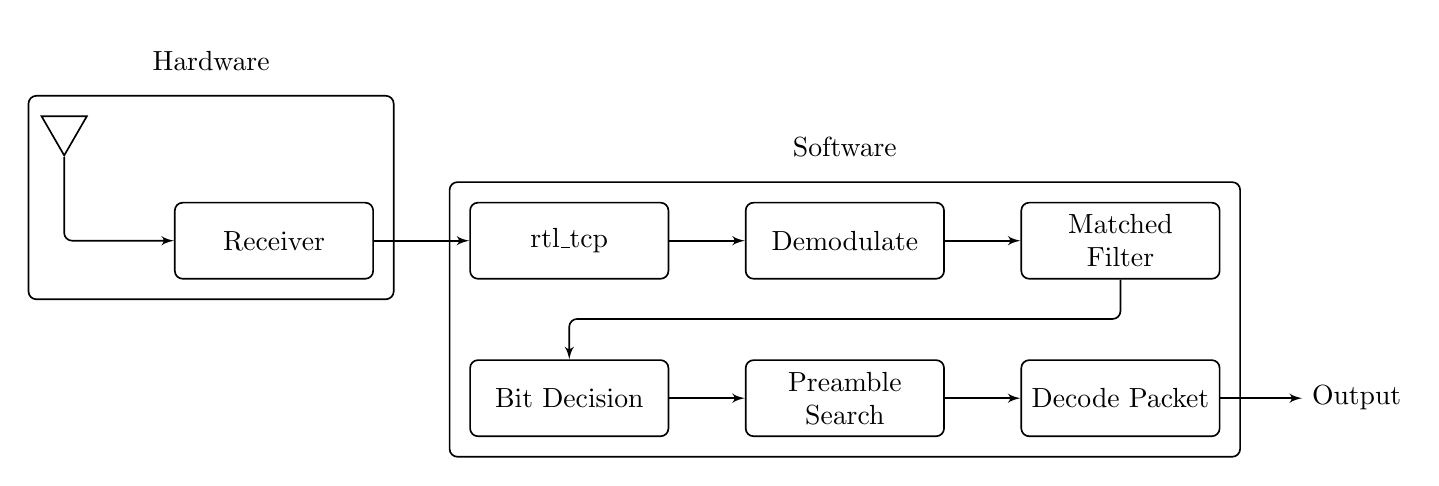
\begin{tikzpicture}[semithick, rounded corners=1mm]
		\node[draw, regular polygon,regular polygon sides=3, rotate=180, rounded corners=0] (antenna) {};
		\node [punkt, below right of=antenna, node distance=2cm, xshift=1.25cm] (rtl-sdr) {Receiver};
		\node [punkt, right of=rtl-sdr, node distance=3.75cm] (rtl-tcp) {rtl\_tcp};
		\node [punkt, right of=rtl-tcp] (demodulate) {Demodulate};
		\node [punkt, right of=demodulate] (filter) {Matched Filter};
		\node [punkt, below of=rtl-tcp, node distance=2cm] (decision) {Bit Decision};
		\node [punkt, right of=decision] (preamble) {Preamble Search};
		\node [punkt, right of=preamble] (decode) {Decode Packet};
		\node [right of=decode, xshift=-0.5cm] (output) {Output};

		\draw [->] (antenna) |- (rtl-sdr);
		\draw [->] (rtl-sdr) -- (rtl-tcp);
		\draw [->] (rtl-tcp) -- (demodulate);
		\draw [->] (demodulate) -- (filter);

		% $(u1.east) + (0.1cm, -0.4cm)$
		\draw [->, rounded corners=1mm] (filter.south) -- ++(0, -0.5cm) -| (decision.north);

		\draw [->] (decision) -- (preamble);
		\draw [->] (preamble) -- (decode);
		\draw [->] (decode) -- (output);

		\node [punkt] (hardware) [fit=(antenna) (rtl-sdr), inner sep=0.25cm] {};
		\node at (hardware.north) [above, inner sep=3mm] {Hardware};

		\node [punkt] (software) [fit=(rtl-tcp) (decode), inner sep=0.25cm] {};
		\node at (software.north) [above, inner sep=3mm] {Software};
	\end{tikzpicture}
\end{document}